%! Author = julianmour
%! Date = 01/05/2023

\section{Preliminary Results}
We evaluated our preliminary approach on the MNIST dataset, consisting of images showing a singular digit.
The classifier's goal is to return the correct classification of a given digit. Specifically we checked the the robustness of class $c=0$.

We evaluated our algorithm against three different scenarios using three different models: a fully connected network 3X10, and two convolutional neural networks with different number of iterations during training. For each model, noted as $D$, we defined encoded our problem definition using MIPVerify ~\cite{MIPVERIFY}, where $F_1$ is $D$ and $F_2$ is also $D$ with a slight change in a singular weight in the last layer on $D$. MIPVerify returns the bounds for the confidence and the time it took to solve. The timeout was set to 50800 seconds. We compared between two approaches for each model:
\begin{itemize}
    \item Solving the confidence bounds without the proposed constraints, noted as "Baseline".
    \item Solving the confidence bounds using the proposed constraints, noted as "Our approach".
\end{itemize}
The preliminary results show a significant improvement of 82\% in execution time when applying the second approach.
The bounds for the confidence were similar in both of the approaches.
Although the results show the improvement in salability of our approach, it is only tested on a specific scenario of two almost identical networks, besides a singular weight.
\begin{figure}[ht]
  \centering
  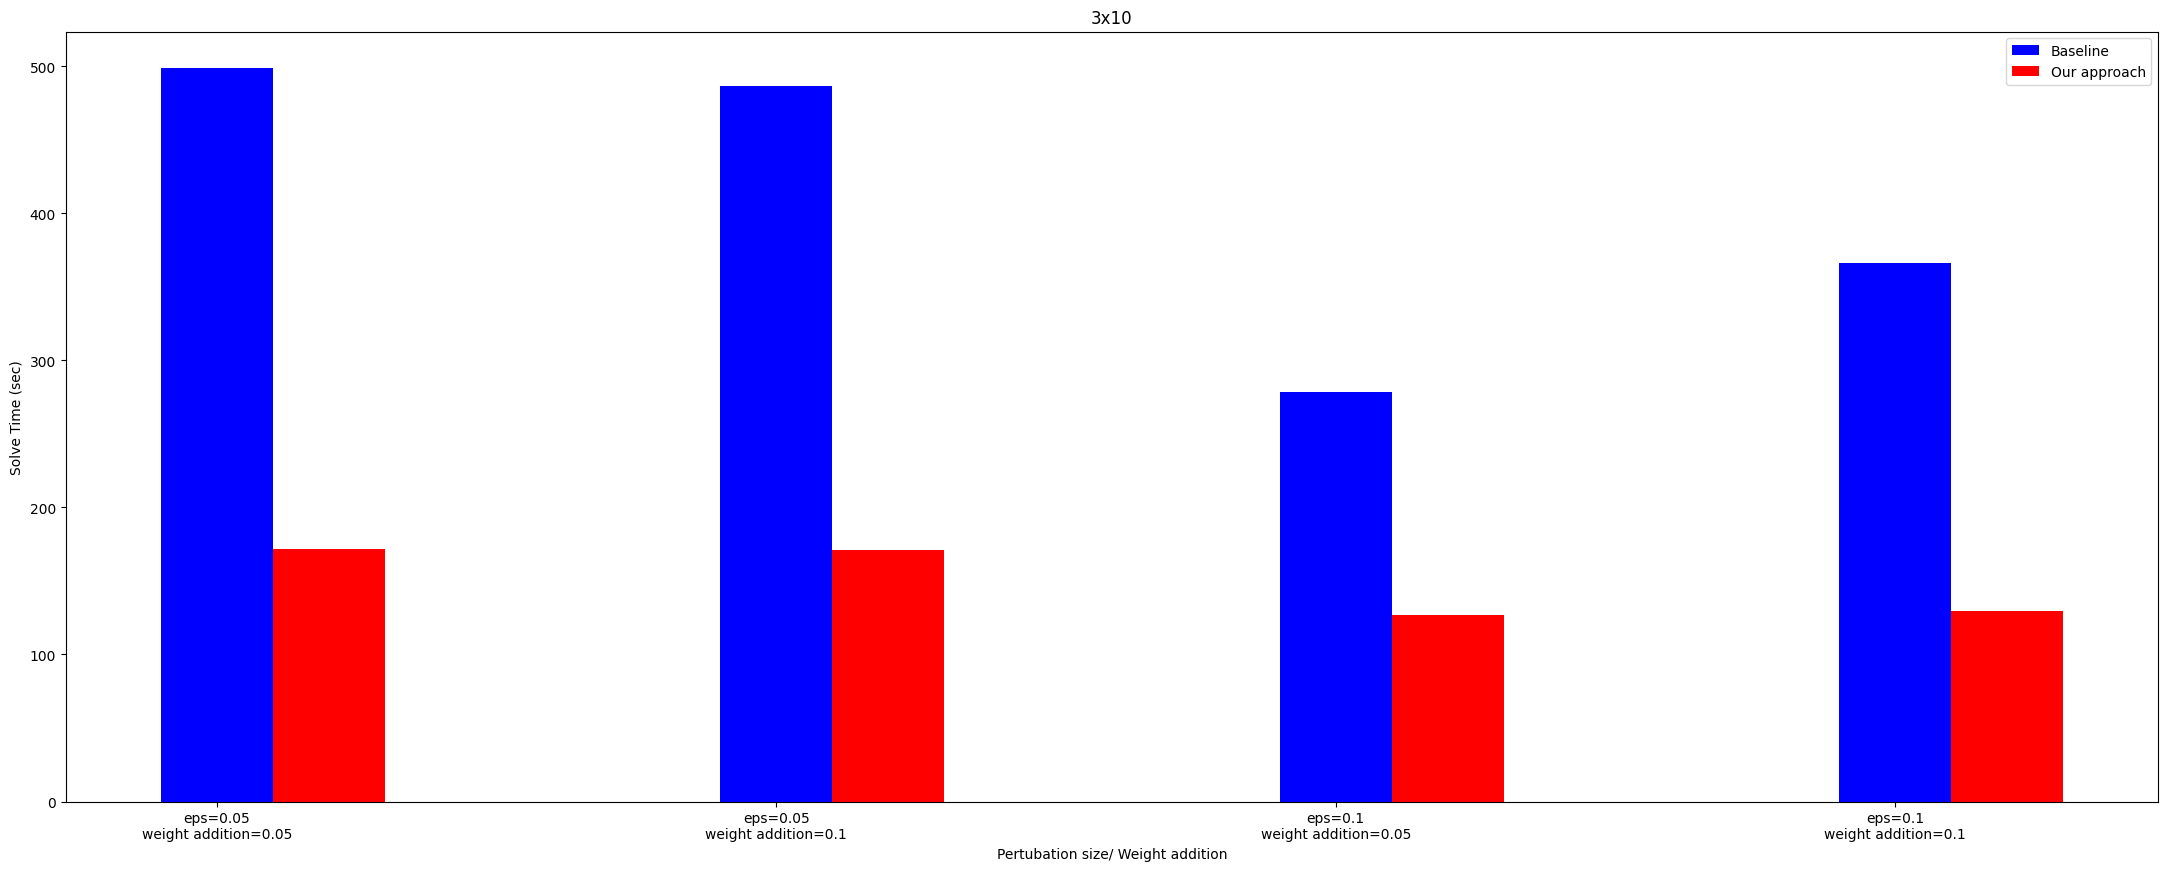
\includegraphics[width=0.95\textwidth]{3x10.png}
  \caption{The execution time of the baseline against our approach, when the model type is a fully connected network 3x10 .}
  \label{fig:3_x_10}
\end{figure}

\begin{figure}[ht]
  \centering
  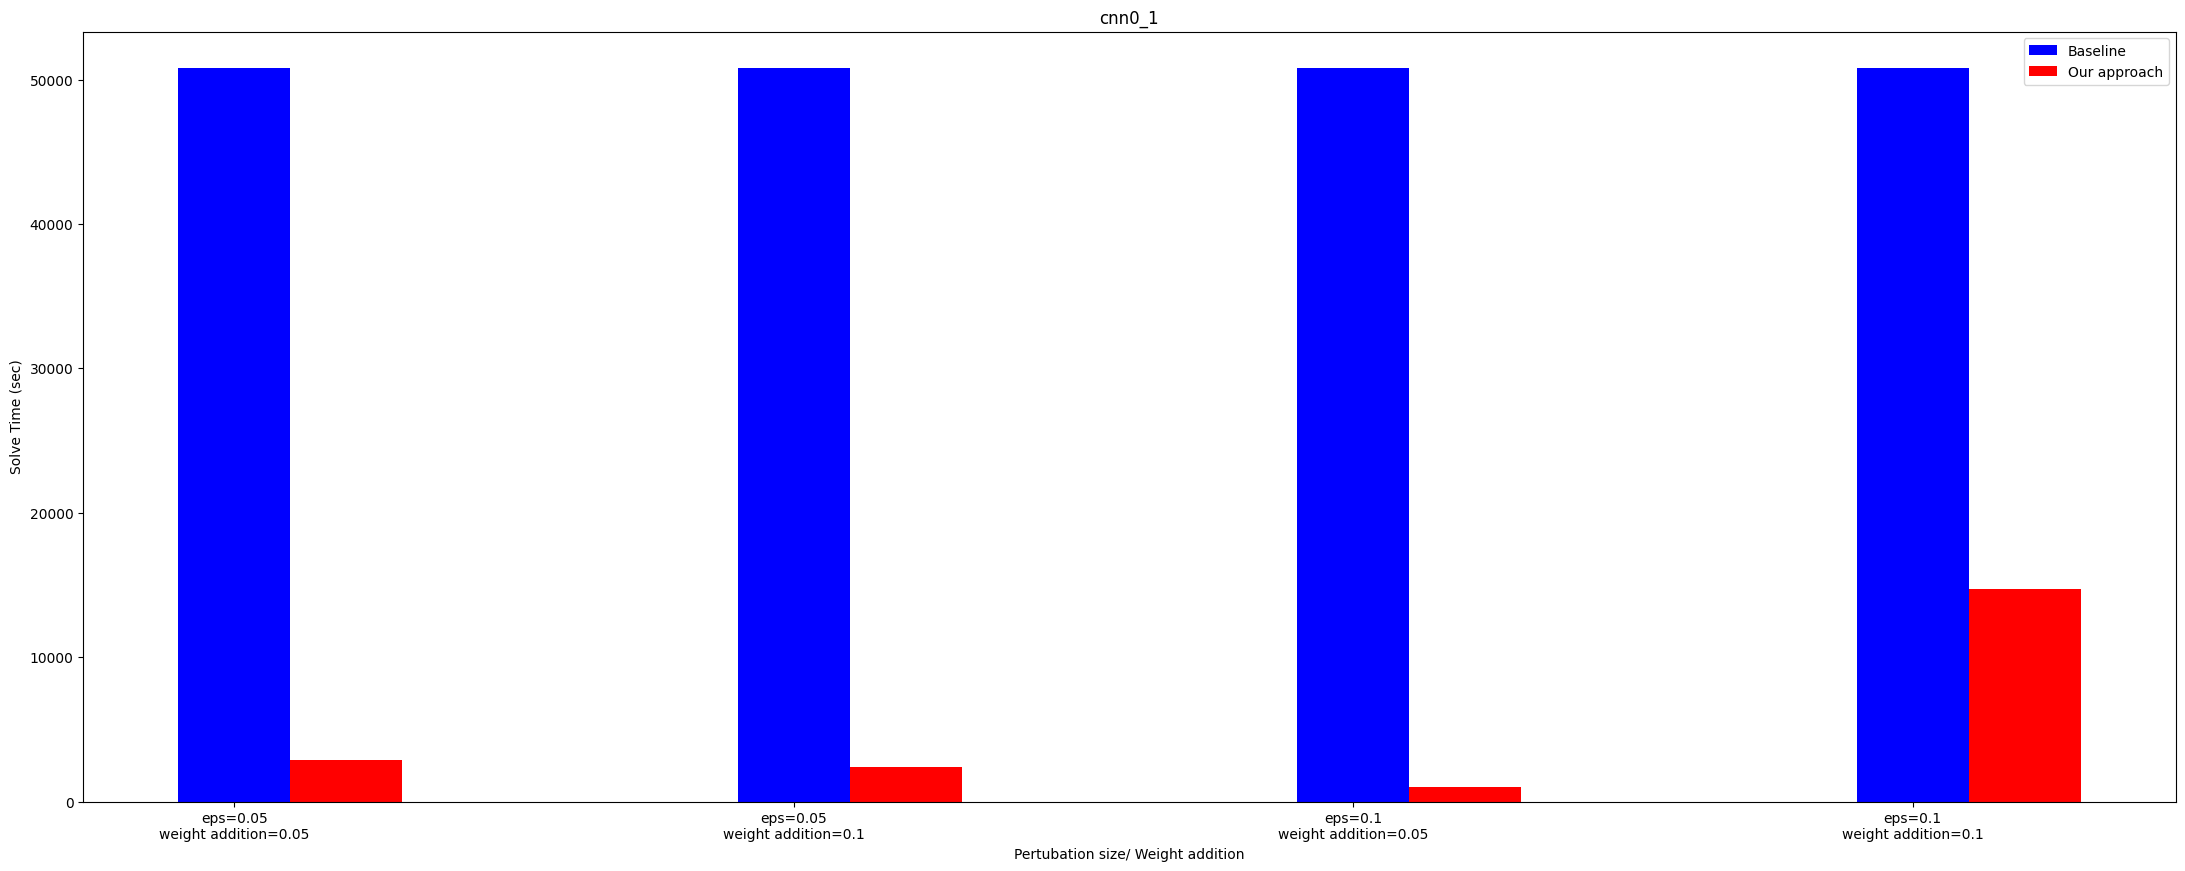
\includegraphics[width=0.95\textwidth]{cnn0_1.png}
  \caption{The execution time of the baseline against our approach, when the model type is a convolutional neural network, trained using 20 iterations .}
  \label{fig:cnn0_1}
\end{figure}

\begin{figure}[ht]
  \centering
  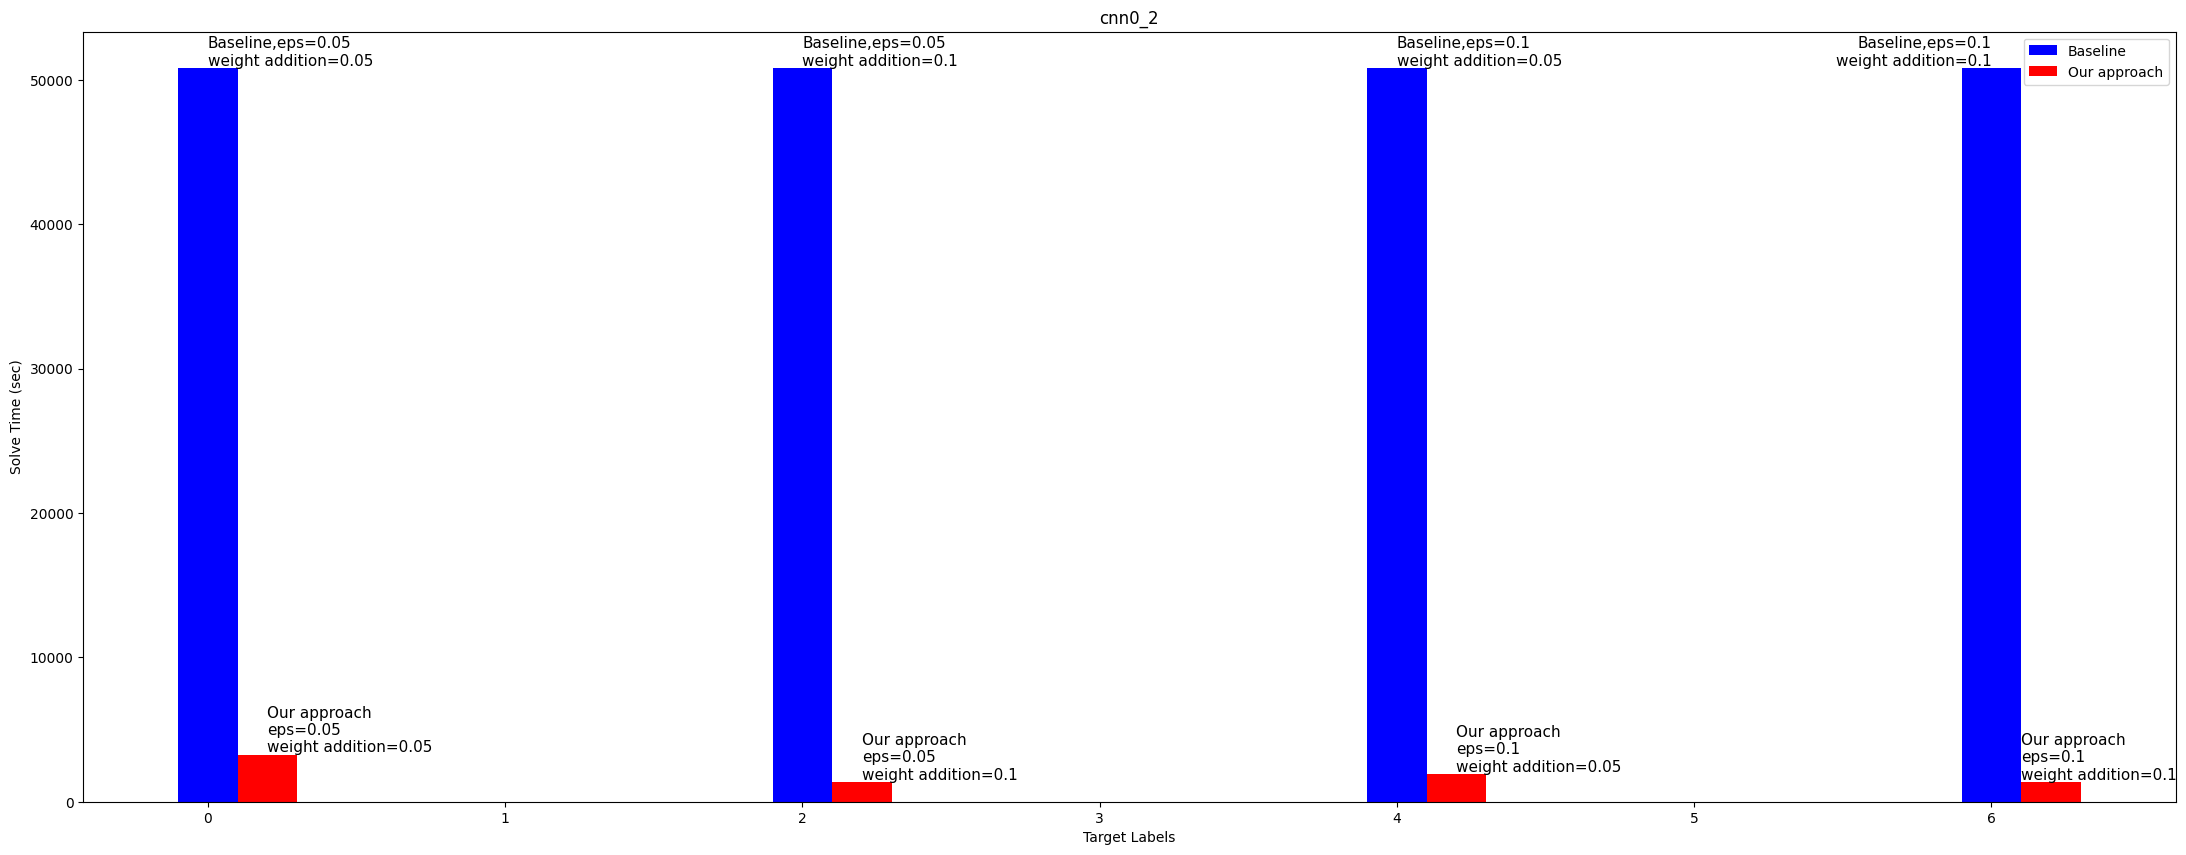
\includegraphics[width=0.95\textwidth]{cnn0_2.png}
  \caption{The execution time of the baseline against our approach, when the model type is a convolutional neural network, trained using 19 iterations .}
  \label{fig:cnn0_2}
\end{figure}

% NETA - image of database + explain: "hey we did good - but not good enough". 

% bounds in table
% times show in graph 